
\section{Introduction}
%The study of the polarization of the cosmic microwave background will bring additional information about both the gravitational and matter sectors of the primordial universe. However, for primordial gravitational waves there are clear theoretical thresholds that can be reached with this next generation instrument. We will use the tensor-to-scalar ratio as the primary inflationary science driver for the design.

With departures from complete homogeneity and isotropy at the $10^{-5}$ level and smaller, given a model, the statistical properties of temperature and polarization anisotropies of the CMB can be calculated to extremely high accuracy using perturbation theory. Their observation thus provides us with an opportunity for comparison with theory with a minimal amount of theoretical (calculational) uncertainty. The CMB provides us with a laboratory for the precision study of the origin of these small perturbations, which in turn is the study of the origins of all structure in the universe.

To date we have observed the result of {\em scalar} perturbations to the spacetime metric tensor. From these observations we have learned that the primordial scalar perturbations were nearly (but not quite) scale-invariant in the variance of their amplitudes, were consistent with Gaussianity, and, were made up of Fourier modes that all began their subhorizon dynamical evolution with the same temporal phase. 

These conclusions are also the predictions of the simplest models of cosmological inflation, and therefore the observations to date are a major success of the inflationary paradigm. 

But many questions remain. Did inflation actually occur? Are ground-state fluctuations truly the source of density perturbations? If inflation did occur, how did it occur? Was there a single effective field dominating the dynamics of both the background expansion and the perturbations, or were multiple fields involved? What is the connection of inflation physics to the rest of physics?

With CMB-S4 we have an opportunity to open up an entirely new window on the mechanism of the creation of these primordial perturbations: the {\em tensor} sector. We wish to stress the value of this new window in a model-independent manner, while simultaneously using the context of 
inflation to provide a more concrete framework for understanding the implications of the measurement of tensor perturbations. In the context of inflation, this new window offers a more direct probe of the dynamics of the inflationary expansion because the tensor perturbations are an inevitable consequence of the degrees of freedom of the spacetime metric obeying the uncertainty principle. The amplitude of the tensor perturbations depends only on the rate of expansion during inflation. In contrast, the amplitude of the scalar perturbations depends on both the amplitude and slope of the effective potential of the field responsible for inflation, and more generally on the sound speed of the inflaton field as well.

In addition to probing the origin of all structure in the universe, opening the tensor sector also opens up a probe of physics at length scales $\sim 10^9$ times smaller than those probed at the LHC. This small length scale is the size of the future horizon during inflation if it takes place at sufficiently high energies for us to observe the resulting tensor fluctuations. It is accessible because the immense amount of expansion during and since the inflationary epoch magnifies
these small length scales to ones of astrophysical size. If the tensor perturbations are detectable, we are already probing physics at these length scales via the scalar perturbations, but we cannot know this until the tensor perturbations are actually detected.

To date we only have upper limits on the amplitude of tensor perturbations, upper limits that are as strong as they can be from measuring temperature anisotropies. To detect the tensor perturbations we need to improve measurements of CMB polarization. On degree scales a polarization pattern known as B-mode polarization would reveal the existence of primordial tensor modes or gravitational waves. In the tensor sector, CMB-S4 will improve current constraints by almost two orders of magnitude. This is especially interesting because it allows this next generation instrument to reach theoretically well-motivated thresholds for the tensor-to-scalar ratio (the ratio of power in tensor modes to power in scalar modes), which consequently serves as the primary inflationary science driver for the design. 

Inflation predicts B-mode fluctuations  sourced by primordial gravitational waves. But more generally, the B-mode signal again carries information about both the spectrum of primordial perturbations in the tensor (and vector) components of the metric and any physics that affected the evolution of those modes once they re-entered the horizon.  

{\it A detection of primordial gravitational waves would open a completely new window on the physical processes of the early universe and reveal a new scale of particle physics far above those accessible with terrestrial particle colliders. }

If the overall amplitude of the B-mode signal is large enough to be detected at high significance by the CMB S4 instrument, we will be able to begin further characterizing the statistics of the perturbations. Investigating the scale-dependence of the amplitude of fluctuations and their Gaussianity will allow us to determine if the signal is consistent with the amplification of quantum vacuum fluctuations of the metric during inflation. If CMB S-4 measurements are consistent with a nearly scale invariant and a weakly non-Gaussian spectrum, a detection would
\begin{itemize}
 \item Identify the energy scale of inflation. 
  \item Provide strong evidence that gravity is quantized, at least at the linear level.
 \item Provide strong evidence that the complete theory of quantum gravity must accommodate a Planckian field range for the inflaton.
\end{itemize}

Departures from a nearly scale-invariant, Gaussian spectrum would reveal new physics beyond the simplest inflationary models. Existing models propose some examples of predictions from a richer inflationary or post-inflationary sector, which would be tested. However, given the lack of observational constraints on physics at such high energy scales there is also enormous discovery potential. Polarization data also provides consistency checks on the current dominant theoretical framework, including model-independent constraints on the graviton mass and constraints on alternatives to inflation.

In the absence of a detection, CMB-S4 would put some of the most significant constraints on inflation models to date, ruling out large classes models. {\bf What else should be stated here?}

{\bf Insert paragraph emphasizing inflation-related gains from the scalar sector with CMB-S4.}

In Section~\ref{sec:basics} we provide a basic introduction of the inflationary paradigm in its simplest form. In Section \ref{sec:detection} we review in detail what a detection of primordial gravitational waves would mean and what follow-up measurements should or could be done to further characterize any signal. Section \ref{sec:upperLimits} explains the implications of a robust upper limit of $r<0.001$. Section \ref{sec:needs} lays out what is required to achieve that goal. The final two sections describe the significant gains CMB-S4 will allow in constraining other aspects of the primordial universe, both standard and more speculative. These include characterizing the scalar power spectrum, constraining curvature, non-Gaussianity, isocurvature modes, further probes of CMB `anomalies' and tests/constraints of cosmic strings.
 

%Recent reviews \cite{Kamionkowski:2015yta}.

\section{Basics of Cosmological Inflation}
\label{sec:basics}

Inflation is, by definition, a period of accelerating expansion. As explained in Fig.~\ref{fig:PTfigs}, an accelerating universe has a causal structure very different from that of a decelerating universe. In a decelerating universe, a pair of separated comoving particles evolves from being causally disconnected -- in which case the particles, unable to influence each other, are said to be superhorizon -- to being causally connected, or subhorizon. In an accelerating universe, the opposite occurs. In the inflationary scenario, the universe undergoes an accelerating stage, which is followed by a long period of deceleration.


\begin{figure}[ht]
\centering
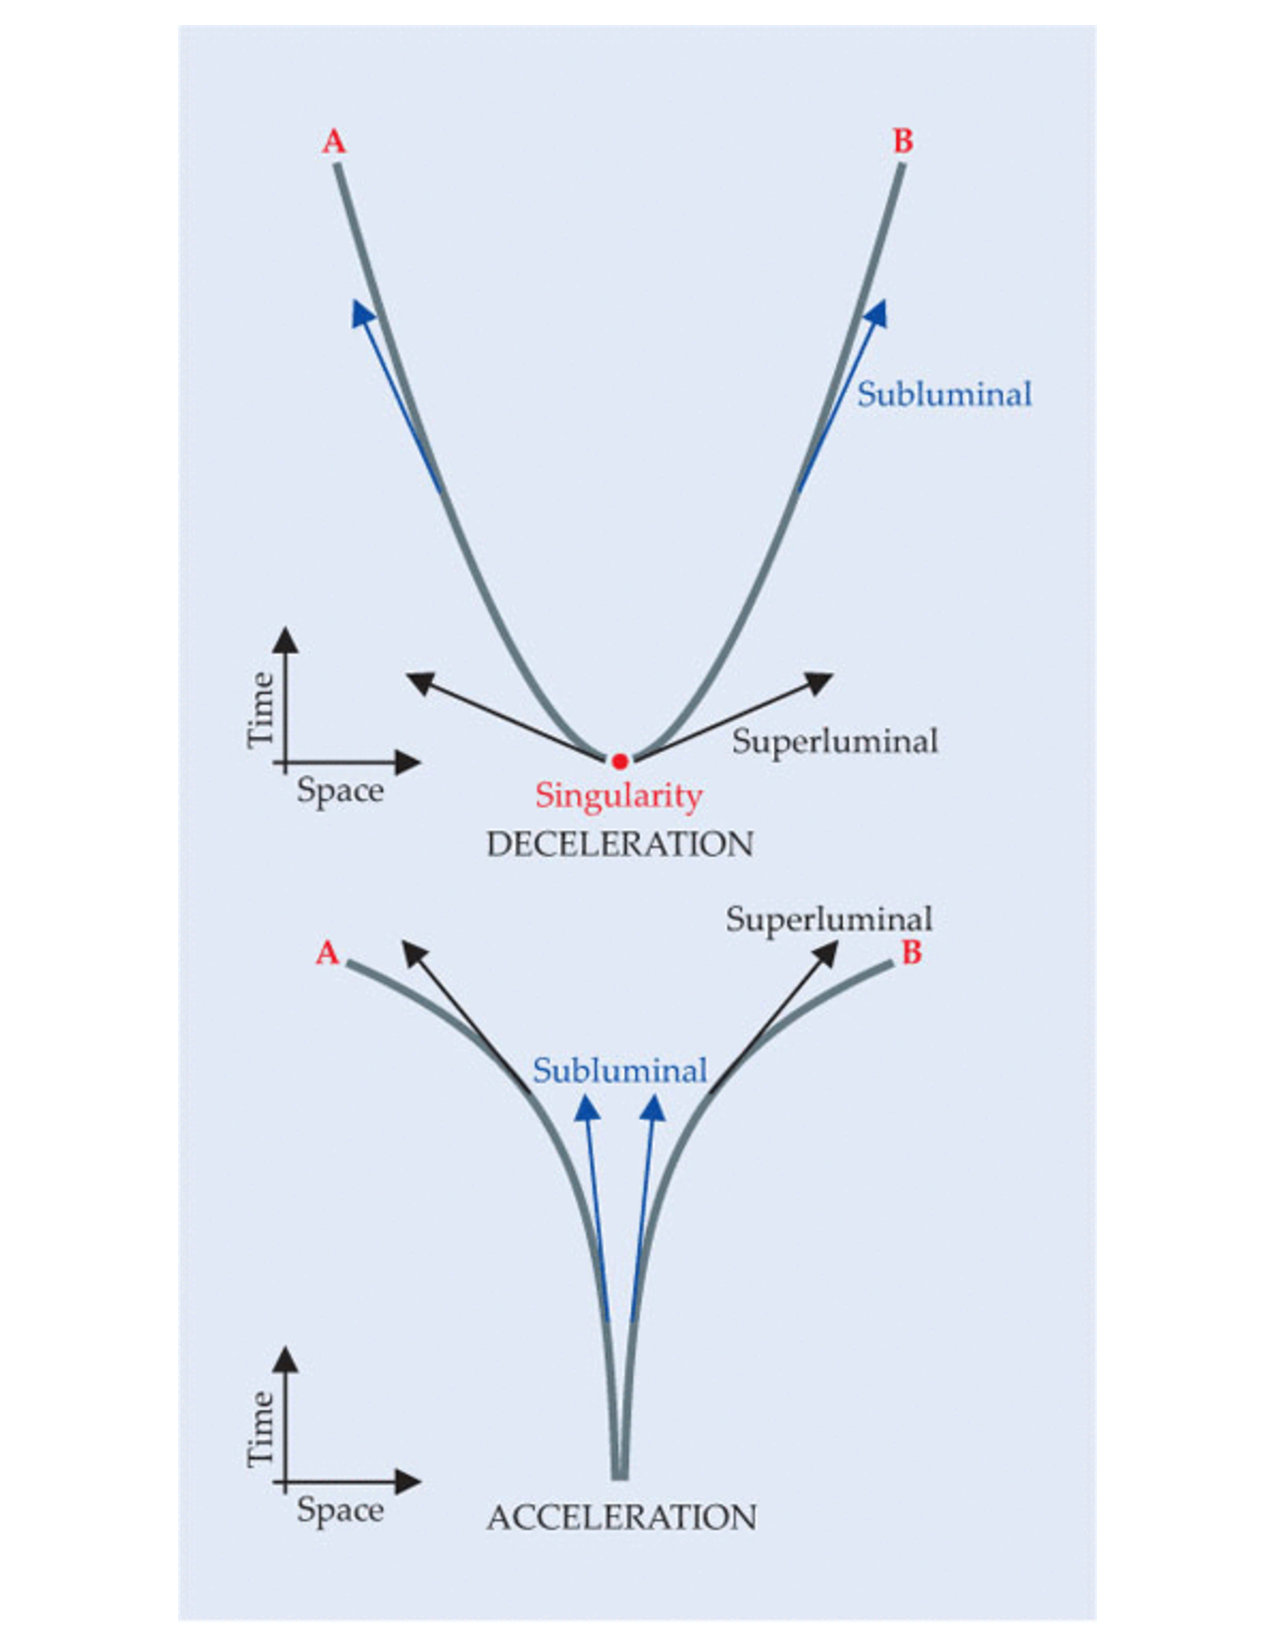
\includegraphics[width=0.36\textwidth]{Inflation/CausalStructure.pdf}
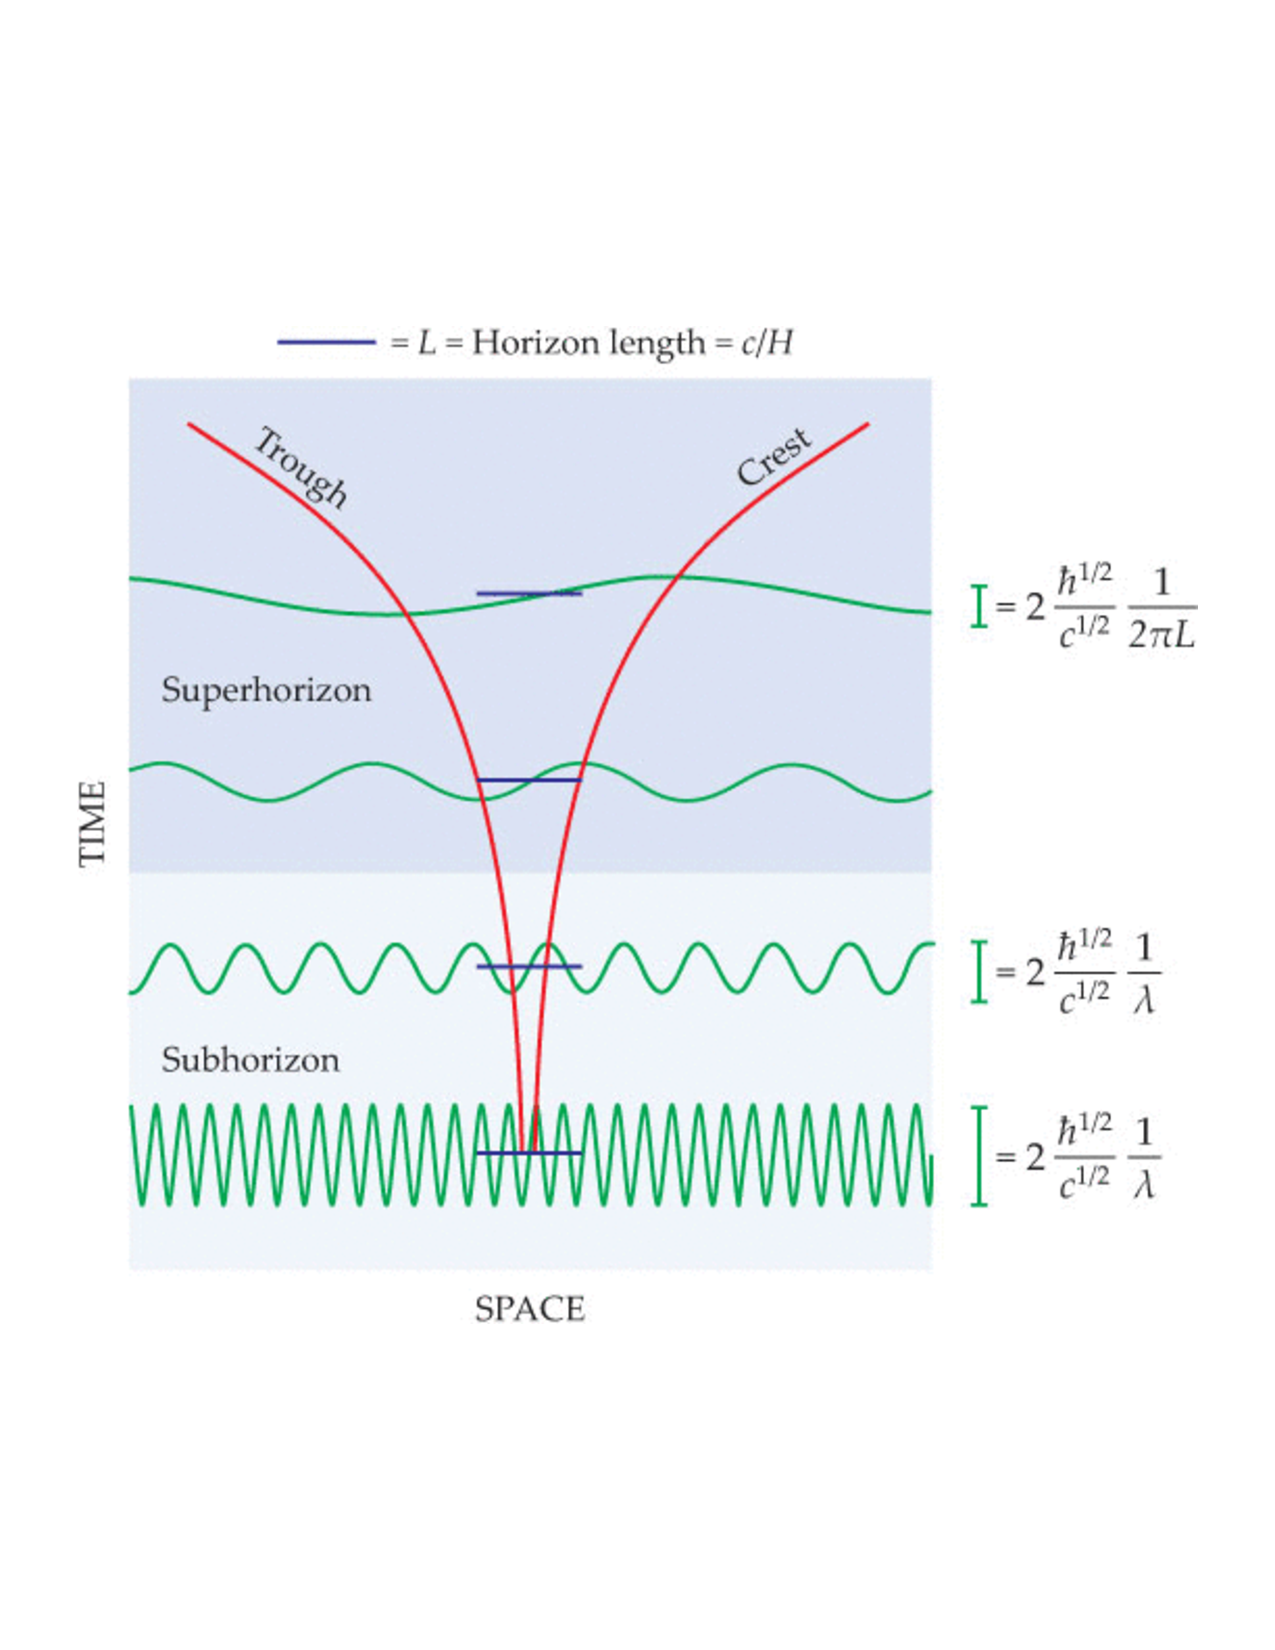
\includegraphics[width=0.36\textwidth]{Inflation/QuantumFluctuations.pdf}
\caption{{\bf Left panel}: In an expanding universe, the distance between two separated points increases over time, simply due to the expansion of the space between them. The two panels here show the spacetime trajectories of two comoving points, A and B. For the decelerating expansion illustrated in the top panel, the separation rate is greater in the past and even exceeds the speed of light at sufficiently early time. Thus A and B go from being out of causal contact—unable to influence each other—to being in causal contact. In an accelerating universe, the separation rate is smaller in the past; the two points go from being in causal contact to being out of causal contact. In the inflationary universe scenario, an early epoch of acceleration—the inflationary era—smoothly maps onto a long period of deceleration. Thus two points can go from being in causal contact to out of causal contact and, much later, back into causal contact. {\bf Right panel}:
Fluctuations in the value of the inflaton field, which is responsible for the accelerating expansion of the cosmos, evolve differently, depending on whether their wavelength $\lambda$ is less than or greater than the horizon length $L = c/H$. When $\lambda \ll L$, the uncertainty principle limits how smooth the field can be. As a result, the amplitude of the fluctuation is inversely proportional to $\lambda$ and thus decreases as the universe expands. (The influence of the uncertainty principle is reflected by the appearance of Planck’s constant $\hbar$ in the expression for the amplitude.) As $\lambda$ becomes larger than the horizon, the crest and trough of the wave cease to be in causal contact, so the amplitude stops evolving. For superhorizon evolution, its asymptotic value corresponds to replacing the wavelength in the subhorizon case with $2\pi L$. Eventually, cosmic expansion stretches the fluctuations to astrophysically large length scales.
}
\label{fig:PTfigs}
\end{figure}


In view of the early period of accelerating expansion, two separated regions in the universe that are now causally disconnected could have been able to interact with each other during the inflationary epoch. Causally connected perturbations in those two regions -- for example, an underdensity in one and an overdensity in the other -- could thus have been created at very early times. Quantum mechanics provides a mechanism for generating such perturbations, and in fact makes them unavoidable. Quantum mechanical fluctuations initially created with subnuclear wavelengths are stretched by the cosmic expansion to millimeter length scales within a tiny fraction of a second; at present they are astrophysically large. Thus observations of cosmic structure give us an opportunity to probe physics on extremely small length scales.

Accelerating expansion requires the universe to have an energy density that dilutes relatively slowly with expansion. In inflationary models, such an energy density is usually obtained via the introduction of a new field $\phi$, called the inflaton field with Lagrangian density, in the simplest cases, given by
\begin{equation}
{\cal L} = \frac{1}{2} \partial_\mu \phi \partial^\mu \phi - V(\phi)
\end{equation}
where $V(\phi)$ is a potential energy density. 

A generic inflaton field configuration will not lead to inflation. But if there is a large enough patch of space in which $\phi$ takes values for which the potential is sufficiently flat, $\phi$ will rapidly evolve to satisfy the ``slow-roll condition'', $\frac{1}{2} \left(d\phi/dt\right)^2 \ll V(\phi)$. When both the spatial and temporal derivatives of the inflaton field are small, $V(\phi)$ is nearly constant in time and makes the dominant contribution to the energy density. Under such conditions, and given the Friedmann equation $\dot a/a \propto \sqrt{\rho}$, the patch inflates. In the limit that the energy density is completely constant in time, the scale factor grows as $e^{H t}$, and points separated by more than $c/H$ are causally disconnected.

A standard assumption in the calculation of inflationary perturbation spectra is that the field is as smooth as it possibly can be, and still be consistent with the uncertainty principle. As Fig.~\ref{fig:PTfigs} shows, these fluctuations will be stretched to astrophysically large length scales by cosmic expansion. In an inflationary scenario quantum fluctuations provide the initial seeds of all structure in the universe. 

As $\phi$ rolls toward the potential minimum, $V(\phi)$ eventually becomes smaller than $\frac{1}{2}(d\phi/dt)^2$; the slow-roll condition is no longer met, and inflation ends. Decays of the inflaton to other particles -- irrelevant during inflation because the decay products were quickly diluted by expansion -- then become important. The remaining energy in the $\phi$ field converts to a thermal bath of the particles of the standard model, and perhaps other particles as well.

The small but nonzero spatial fluctuations in $\phi$ cause inflation to end at different times in different locations. In those regions where inflation ends relatively early, the mass density is lower due to the extra expansion that the region has undergone since the end of inflation. Thus the slightly different expansion histories of different locations result in density differences; those small density perturbations eventually grow under the influence of gravity to create all the structures we observe in the universe today.

The spacetime metric itself, at least in a linearized treatment, presumably obeys the uncertainty principle as well. As a result, we expect a nearly scale-invariant spectrum of gravitational waves to be produced during inflation as well. Just as with fluctuations of the inflaton field, they obey an uncertainty principle and, in the course of superluminal expansion, have their amplitude set to a value proportional to the Hubble parameter $H$ during inflation. Detecting the influence of that gravitational-wave background on the CMB would allow cosmologists to infer $H$ and hence the energy scale of the inflationary potential; observations of density perturbations, by contrast, provide a relatively indirect look at the inflationary era. As emphasized in the previous section, CMB-S4 is poised to detect, or place interesting upper limits, on the amplitude and spectrum of inflation-produced gravitational waves via their signature in B-mode polarization. 


\section{Implications of a detection of primordial gravitational waves with CMB-S4}
\label{sec:detection}
The overall evolution of the universe is well modeled by a Friedmann-Lema\^{\i}tre-Robertson-Walker line element
\begin{equation}
ds^2=-dt^2+a^2(t)\left[\frac{dr^2}{1-kr^2}+r^2d\Omega^2\right]\,,
\end{equation}
where $k=\pm1$ allows for spatial curvature and the time evolution is specified by the scale factor, $a(t)$. The Hubble parameter, $H=\dot{a}/a$, gives the rate of expansion of the universe. 
%Current data is consistent with a spatially flat universe, and we will assume spatial flatness ($k=0$) for most of the discussion. However, we will return to constraints on the curvature in Section xxx.  

The existence of primordial Helium and the cosmic microwave background radiation provide strong evidence for a hot big bang, a period during which the universe was dominated by radiation before it became dominated by matter and eventually dark energy. In the context of general relativity, observations of the cosmic microwave background furthermore provide strong evidence for a period preceding the hot big bang during which the co-moving Hubble radius, $(a|H|)^{-1}$, was decreasing with time: the measured average CMB temperature and the statistics of the measured anisotropies are the same over regions that otherwise share no causal history. 

%Arguably the most significant discrepancy between the predictions of a generic hot big bang model and our observed sky is the horizon problem: the measured average CMB temperature and the statistics of the measured anisotropies are the same over regions that share no causal history. Models for the primordial universe attempt to give a causal (and ideally also a `natural') explanation for the observed homogeneity on scales greater than a few degrees by postulating an early era where the co-moving Hubble radius, $(a|H|)^{-1}$ is decreasing with time. In an expanding universe this requires an era of accelerated expansion, $\ddot{a}>0$. The matter field that sources this expansion should have equation of state $w\approx -1$, which is minimally provided by a single scalar field whose energy density is predominately determined by its potential.

In an expanding universe a decreasing co-moving Hubble radius requires an era of accelerated expansion, $\ddot{a}>0$, cosmic inflation. Such a period will drive the spatial curvature close to zero, in good agreement with current observations. Thus, we will assume spatial flatness and set $k=0$ for most of the discussion, but will return to constraints on the curvature in Section \ref{sec:other_topics}. Since the period of cosmic inflation must end, there must exist a clock, or scalar degree of freedom. According to the uncertainty principle this clock must fluctuate, generating density perturbations that are adiabatic. In the most economic scenarios, these density perturbations are the seeds that grow into the anisotropies observed in the cosmic microwave background radiation and the stars and galaxies around us. Other degrees of freedom could, of course, also be present during this phase and might even be responsible for the generation of density perturbations we observe. 

%{\bf (Mention isocurvature modes here?)}

Alternatively, the phase of decreasing co-moving Hubble radius could have occurred during a period of decelerating contraction which must then be followed by a bounce as in the ekpyrotic or matter bounce scenarios \cite{Khoury:2001wf,Khoury:2001bz,Steinhardt:2001st,Nayeri:2005ck,Brandenberger:2012zb,Cai:2014jla,deHaro:2015wda}. 
% The matter field that sources this expansion should have an equation of state $w\approx -1$, which is minimally provided by a single scalar field whose energy density is predominately determined by its potential.

%The remarkable feature of inflation is that once an evolving scalar field is invoked to source the background accelerated expansion, quantum fluctuations during inflation inevitably generate post-inflationary metric perturbations. 
For these early times, the ADM formalism provides a convenient parametrization of the line element
\begin{eqnarray}
\label{eq:metric}
ds^2&=&-N^2dt^2 +h_{ij}(dx^i+N^idt)(dx^j+N^jdt)\,\nonumber\\
h_{ij}&=&a^2(t)[e^{2\zeta}\delta_{ij}+\gamma_{ij}]\,.
\end{eqnarray}

The equations of motion for $N$ (the lapse) and $N^i$ (the shift) are the Hamiltonian and momentum constraints, while $\zeta$ ($=-\mathcal{R}$ in the {\it Planck} collaboration papers) and $\gamma_{ij}$ contain the dynamical scalar and tensor degrees of freedom. In scenarios with matter sources other than a scalar field there may also be vector perturbations. These rapidly decay and can be neglected unless they are actively sourced in the post-inflationary universe, e.g. by cosmic strings.

%RF perhaps add Fourier transform and define horizon exit, freeze out at this point
Because the equations of motion are invariant under translations and the perturbations are linear or nearly so, it is convenient to work with the Fourier transforms
\begin{equation}
\zeta(t,\vec{x})=\int \frac{d^3 k}{(2\pi)^3}\zeta(t,\vec{k})e^{i \vec{k}\cdot\vec{x}}+h.c.\qquad{\rm and}\qquad\gamma_{ij}(t,\vec{x})=\sum\limits_s\int\frac{d^3k}{(2\pi)^3}\gamma_s(t,\vec{k})e_{ij}(\vec{k},s)e^{i \vec{k}\cdot\vec{x}}+h.c.\,,
\end{equation}
where $e_{ij}(\vec{k},s)$ is the transverse traceless polarization tensor for the graviton. The solutions oscillate when the modes are deep inside the horizon, $k\gg aH$. By definition, the modes exit the horizon when $k=aH$ and in single-field models approach a constant outside the horizon when $k\ll aH$.

The statistical properties of the scalar and tensor fluctuations, $\zeta$ and $\gamma_s$, at times sufficiently late so that they have frozen out provide the link between the primordial era and the observed CMB today as well as other probes of the structure of the late universe. For a universe that is statistically homogeneous and isotropic and in which the primordial fluctuations are Gaussian, the information about the statistical properties is contained in the two-point correlation functions

\begin{eqnarray}
\langle\zeta(\vec{k})\zeta(\vec{k}^{\prime})\rangle&=&(2\pi)^3\delta^3(\vec{k}+\vec{k}^{\prime})\frac{2\pi^2}{k^3}\mathcal{P}_{\zeta}(k)\nonumber\\
\langle\gamma_s(\vec{k})\gamma_{s^{\prime}}(\vec{k}^{\prime})\rangle&=&(2\pi)^3\delta_{ss^{\prime}}\delta^3(\vec{k}+\vec{k}^{\prime})\frac{2\pi^2}{k^3}\frac{1}{2}\mathcal{P}_{t}(k)\nonumber\\
\end{eqnarray}
where the factor of $1/2$ in the second to last line accounts for the fact that the measured power includes contributions from each of the two graviton polarizations. In single field slow-roll inflation, the gauge invariant combination of metric and scalar field fluctuations that is conserved outside the horizon has the power spectrum
\begin{equation}
\label{eq:inf_Pzeta}
\mathcal{P}_{\zeta}(k)=\frac{1}{2\epsilon M_p^2}\left.\left(\frac{H}{2\pi}\right)^2\right|_{k=aH}
\end{equation}
where $\epsilon=-\dot{H}/H^2$ is the first slow-roll parameter, and $M_p=1/\sqrt{8\pi G}$ is the reduced Planck mass. As indicated, the Hubble parameter and $\epsilon$ are to be evaluated at horizon exit when the wavenumber $k$ is equal to the inverse comoving Hubble radius. In the absence of additional sources, the tensor power spectrum generated by inflation is
\begin{equation}
\label{eq:inf_Pt}
\mathcal{P}_{t}(k)=\frac{8}{M_p^2}\left.\left(\frac{H}{2\pi}\right)^2\right|_{k=aH}
\end{equation}

It is convenient to introduce the logarithmic derivatives of these power spectra 
\begin{equation}\label{eq:specind}
n_s(k)-1\equiv\frac{d\ln \mathcal{P}_{\zeta}}{d\ln k}\qquad{\rm and}\qquad n_t(k)\equiv \frac{d\ln \mathcal{P}_t}{d\ln k}\,.
\end{equation}
If the Hubble rate and slow-roll parameter only weakly depend on time as in slow-roll inflation, these will be $n_s(k)\approx 1$ and $n_t(k)\approx 0$ and can be expanded around a pivot scale $k_\star$ accessible by the CMB
\begin{equation}
n_s(k)-1=n_s-1+\left.\frac{dn_s(k)}{d\ln k}\right|_{k_\star}\ln(k/k_\star)+\dots\qquad{\rm and}\qquad n_t(k)=n_t+\left.\frac{dn_t(k)}{d\ln k}\right|_{k_\star}\ln(k/k_\star)+\dots
\end{equation}
In this approximation, the power spectra are
\begin{eqnarray}\label{eq:power_spectra_power_law}
\mathcal{P}_{\zeta}(k)&=& A_s\left(\frac{k}{k_\star}\right)^{n_s-1+\frac{1}{2}\left.\frac{dn_s}{d\ln k}\right|_{k=k_\star}\ln(k/k_\star)+\dots}\,,\nonumber\\
\mathcal{P}_{t}(k)&=& A_t \left(\frac{k}{k_\star}\right)^{n_t+\frac{1}{2}\left.\frac{dn_t}{d\ln k}\right|_{k=k_\star}\ln(k/k_\star)+\dots}\,,
\end{eqnarray}
%\begin{equation}\label{eq:specind}
%\mathcal{P}_{\zeta}(k)\equiv A_s\left(\frac{k}{k_\star}\right)^{n_s-1}\qquad{\rm and}\qquad\mathcal{P}_{t}(k)\equiv A_t \left(\frac{k}{k_\star}\right)^{n_t}\,,
%\end{equation}
where $A_s$, $A_t$ are the scalar and tensor amplitudes, and $n_s$ and $n_t$, are the scalar and tensor spectral index, respectively, both at the pivot scale. 
The tensor-to-scalar ratio, $r$, is the relative power in the two types of fluctuations at a chosen pivot scale $k_\star$ accessible by the CMB
\begin{equation}
r=\frac{A_t}{A_s}\;.
\end{equation}

The power spectra of $\zeta$ and $\gamma_s$ are time-independent as long as the modes are outside the horizon, and only begin to evolve once the modes of interest re-enter the horizon at late times. In particular, they set the initial conditions for the system of equations governing the time evolution of the universe from around $10^9$ K when electrons and positrons have annihilated to the present. To exhibit the link between the primordial perturbations and late time observables explicitly, note that in a spatially flat universe, the contributions of primordial scalar perturbations to the angular power spectra of temperature or E-mode anisotropies are given by
\begin{equation}
C^{(S)}_{XX,\ell}=\int \frac{dk}{k}\mathcal{P}_\zeta(k)\left|\int\limits_0^{\tau_0} d\tau S_X^{(S)}(k,\tau)j_\ell(k(\tau_0-\tau))\right|^2\,,
\end{equation}
where $j_\ell$ is a spherical Bessel function that encodes the (spatially flat) geometry of the universe and $S_X^{(S)}(k,\tau)$ with $X=T,E$ are source functions that encode the evolution of the modes in the hot big bang universe (in particular, the physics of recombination is very important for B-modes).
% and $\mathcal{P}_\zeta(k)$ is the power spectrum of initial conditions of primordial scalar perturbations as a function of the (comoving) momentum of the modes. 
At linear order, scalar perturbations only contribute to angular power spectra of temperature and E-mode polarization and the cross-spectrum of temperature and E-mode polarization, while the tensor perturbations in addition generate B-mode polarization. The primordial contribution of the tensor perturbations to the angular power spectrum of B-modes is 
\begin{equation}
C_{BB,\ell}=\int \frac{dk}{k}\mathcal{P}_t(k)\left|\int\limits_0^{\tau_0} d\tau S_B^{(T)}(k,\tau)j_\ell(k(\tau_0-\tau))\right|^2\,.
\end{equation}
where $S_B^{(T)}(k,\tau)$ is the appropriate source function. 

At present, bounds on the tensor contribution to the temperature and E-mode anisotropies are comparable to constraints on the tensor-to-scalar ratio from B-mode observations. The former constraints are now cosmic variance limited. There is no limit on the latter from cosmic variance, and improvements and a potential detection with CMB-S4 will rely on measurements of B-mode polarization on degree scales.

Constraints on the amplitude of primordial tensor modes already strongly disfavor once popular inflationary models like minimally coupled chaotic inflation with a quadratic potential. In the next few subsections we will discuss in detail what a detection of primordial gravitational waves would imply for theories of the primordial universe. 

%but it is also important to note that a detection would rule out contracting universe scenarios. A contracting universe can also put large scales in causal contact if the scale factor $a$ is nearly constant while the magnitude of the Hubble parameter increases. This means the spectrum of gravitational wave fluctuations will be very blue \cite{Khoury:2001wf}. In addition the Hubble parameter at the end of the contracting phase can be approximately bounded (minimally, $H<M_p$, or $H\sim T_{\rm reheat}$) and so the value of $H$ that sets the amplitude of tensor fluctuations on scales accessible through the CMB must be exponentially smaller. The vacuum fluctuations in a contracting universe are then far too small to be detected \cite{Boyle:2003km}.

